%!TEX root = ../main

\newpage
\section{Model parallel \& data parallel}
%\indent\setlength{\parindent}{1em} 
Главными подходами для распределенного обучения нейронных сетей является data-parallel и model-parallel. Однако эти подходы не лишены недостатков. В статье "PipeDream: Fast and Efficient Pipeline Parallel DNN Training"\cite{pipedream} описаны основные проблемы данных подходов и предложена система PipeDream, комбинирующая эти методы и тем самым оптимизирующая их.

\subsection{Data parallelism}
Идея Data parallelism заключается в разбиении исходных данных на части, каждая из которых будет использована на отдельной GPU. На каждой GPU находится своя полная копия Нейронной Сети, и веса, получаемые в ходе обучения, синхронизируются между GPU раз в несколько эпох.


\begin{figure}[h]%current location
	\centering
	\scalebox{0.7}{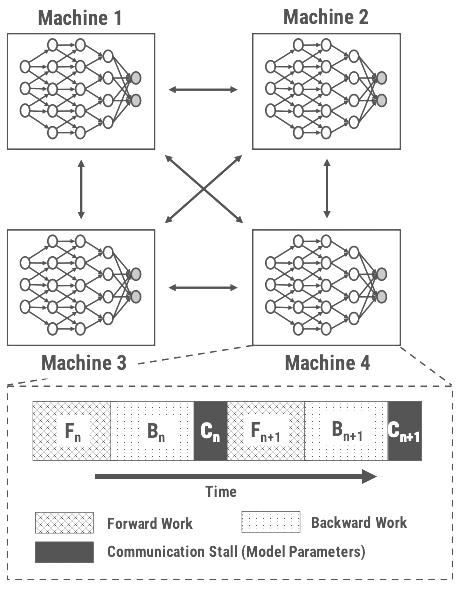
\includegraphics{Parts/images/data-parallel.jpg}}
	\caption{Пример data-parallel на 4 GPU}
	\label{data_parallel} %framework,fig1
\end{figure}


%\indent\setlength{\parindent}{1em} 
Однако главная проблема data-parallel заключена в долгом синхронизировании данных между процессами. Были проведены тесты на различных известных нейронных сетях на трех разных видеокартах NVIDIA GPU -- Kepler (K80), Pascal (Titan X) и Volta (V100), и было замерено время, идущее на синхронизацию между процессами:

\begin{figure}[h]%current location
	\centering
	\scalebox{0.7}{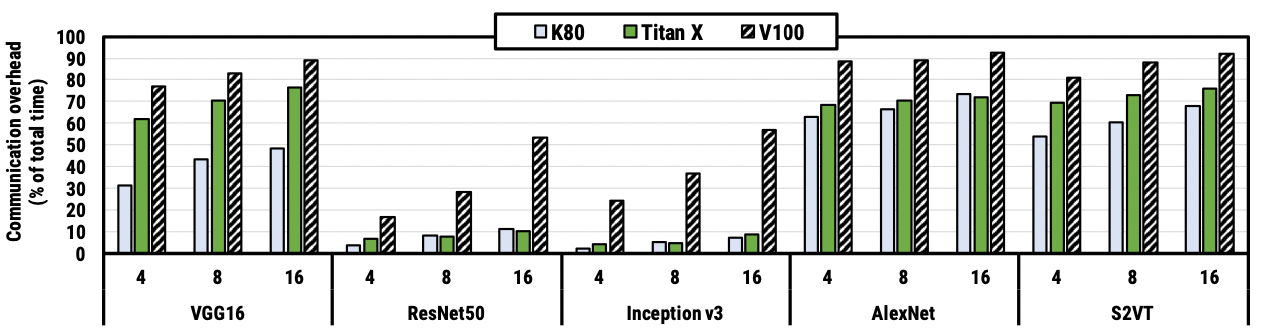
\includegraphics{Parts/images/communication-overhead.jpg}}
	\caption{Время на синхронизацию в \% от всего времени обучения DNN}
	\label{communication_overhead} %framework,fig1
\end{figure}

%\indent\setlength{\parindent}{1em} 
Как видно на данном графике \ref{communication_overhead}, время, занимаемое на синхронизацию , может достигать до 90\% от всего времени обучения DNN.

\newpage
\subsection{Model Parallelism}
Идея Model Parallelism заключается в разбиении самой модели на несколько частей, каждая из которых будет вычисляться на отдельной GPU. Данный подход часто используется в Машинном Обучении (ML). Однако для DNN наивный подход model-parallel имеет огромный недостаток. Разбивая Нейронную Сети на части по несколько слоев Нейронной Сети, отдельная часть должна вычисляться только после вычисления предыдущей части:

\begin{figure}[h]%current location
	\centering
	\scalebox{1}{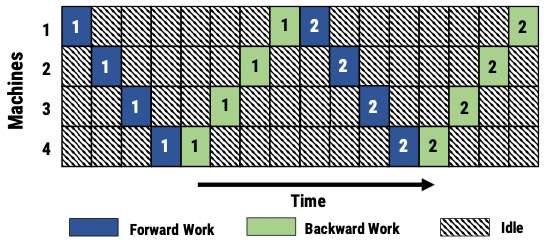
\includegraphics{Parts/images/model-parallel.jpg}}
	\caption{Процесс наивного model-parallel на 4 GPU. \\Числа обозначают номер батча.}
	\label{framework} %framework,fig1
\end{figure}

%\indent\setlength{\parindent}{1em} 
Из-за такого подхода наши GPU значительную часть времени находятся в режиме ожидания, и как такового прироста в производительности нет.

\subsection{PipeDream}
%\indent\setlength{\parindent}{1em}  
PipeDream использует идею model-parallel, деля DNN на части по несколько слоев Нейронной Сети, но при этом, прямые и обратные проходы для разных батчей будут выполянться параллельно, тем самым минимизируя работу GPU в режиме ожидания.

\begin{figure}[h]%current location
	\centering
	\scalebox{1}{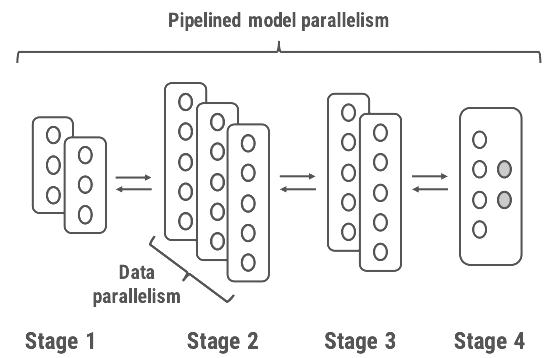
\includegraphics{Parts/images/pipelined_model_example.jpg}}
	\caption{Процесс обучения PipeDream, объединяющий data-parallel и model-parallel}
	\label{framework} %framework,fig1
\end{figure}

\newpage
\subsubsection{Распределение слоев между GPU}

\begin{wrapfigure}[14]{r}{0.5\textwidth}
    \vspace{-2cm}
	\begin{center}
		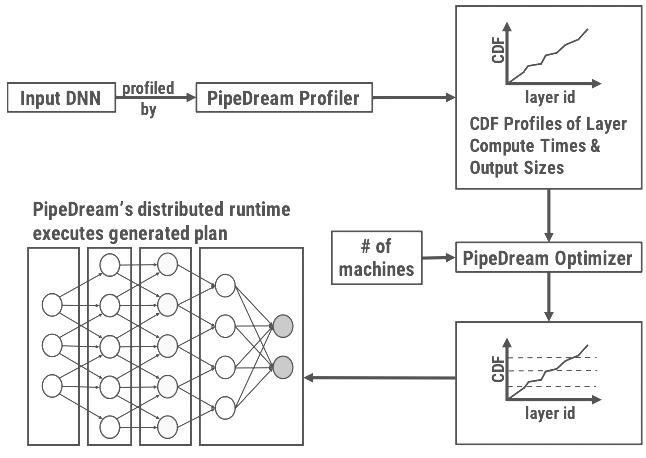
\includegraphics[width=\linewidth]{Parts/images/pipedream_process.jpg}
	\end{center}
	\caption{Автоматизированный процесс деления DNN на части}
    \label{fig:transformer1}
\end{wrapfigure}

%\indent\setlength{\parindent}{1em}  
Для минимизации времени работу GPU в режиме ожидания важно правильно поделить DNN на части. Главная задача при разделении заключается в том, что каждая отдельная компонента PipeDream выполнялась одинаковое количество времени.

Для этого вначале производится замер времени работы DNN, производя вычисления 1000 батчей на одной из GPU. После этого при помощи динамического программирования находится оптимальное разделения на части, каждая из который будет вычисляться одинаковое количество времени (тогда мы можем считать, что каждая часть выполняется ровно одну единицу времени).

% \begin{figure}[h]%current location
% 	\centering
% 	\scalebox{0.7}{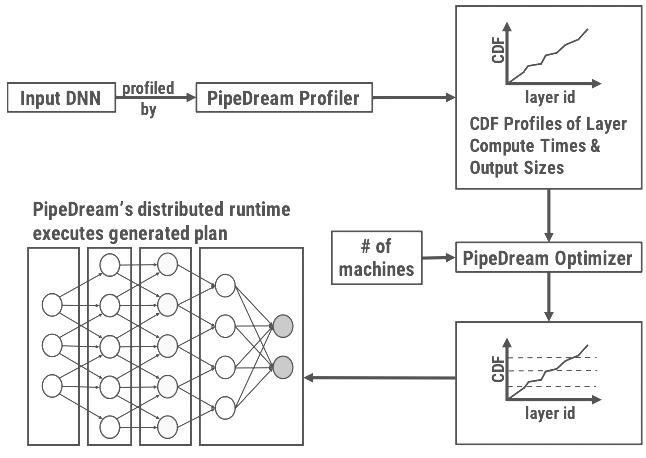
\includegraphics{Parts/images/pipedream_process.jpg}}
% 	\caption{Автоматизированный процесс деления DNN на части}
% 	\label{framework} %framework,fig1
% \end{figure}

\subsubsection{Последовательность вычисления}
%\indent\setlength{\parindent}{1em}
В отличие от обычных реализаций pipeline, в которых одновременно вычисления происходят только либо в прямом, либо в обратном порядке, в PipeDream вычисления происходят в обе стороны одновременно. То есть у каждой GPU в каждую единицу времени есть выбор: либо делать прямой проход графа вычислений, либо обратный. 

\begin{figure}[h]%current location
	\centering
	\scalebox{1}{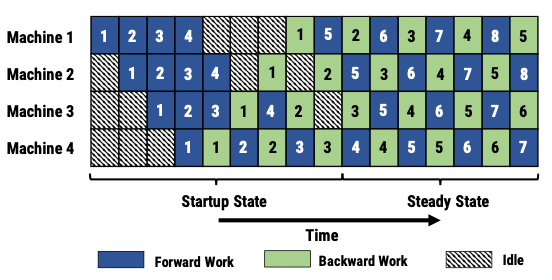
\includegraphics{Parts/images/pipedream_work_schedule.jpg}}
	\caption{Автоматизированный процесс деления DNN на части}
	\label{framework} %framework,fig1
\end{figure}

%\indent\setlength{\parindent}{1em}  
В начальной стадии использнения PipeDream, первая часть получает на вход оптимальное количество батчей, последовательно после вычисления передавая следующей части (а значит и следующей GPU) результат вычисления. 

%\indent\setlength{\parindent}{1em}  
В основной стадии работы PipeDream на одной GPU чередуются прямой и обратный проходы. Такой механизм авторы статьи назвали one-forward-one-backward (1F1B).

\subsubsection{Эффективность обучения}
%\indent\setlength{\parindent}{1em} 
Как мы можем видеть из примера из последней иллюстрации: прямой проход для батча №5 для первой GPU проходит после обновления весов после обратного прохода батча №1. При этом обратный проход батча №5 проходит после оборатных проходов батчей №2, №3 и №4. Это может негативно влиять на сходимость.

%\indent\setlength{\parindent}{1em}
\textbf{Weight Stashing:} в PipeDream реализована идея сохранения весов для всех батчей, которые в данный момент времени вычисляются в модели. Таким образом, когда батчу нужно пройти прямой проход, то используются последняя версия весов. После этого сохраняется версия весов, которая вспоследствии будет использована при обратном проходе того же батча. Такой метод авторы статьи называют Weight Stashing. Благодаря ему для каждой части модели для каждого батча используются подходящие веса, как для прямого, так и для обратного проходов. Тем самым не будет нарушена сходимость графа вычислений.

\subsection{Заключение}
%\indent\setlength{\parindent}{1em} 
PipeDream существенно превосходит метод data-parallel, посколько каждая GPU обменивается только частью параменторв (таким образом синхронизация происходит быстрее):

\begin{figure}[h]%current location
	\centering
	\scalebox{0.7}{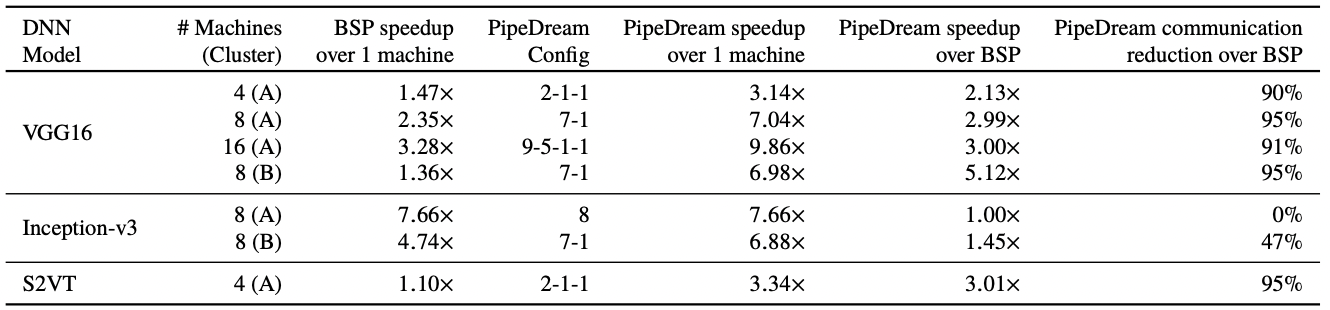
\includegraphics{Parts/images/pipedream_tests.jpg}}
	\caption{Сравнение PipeDream с data-parallelism (BSP)}
	\label{framework} %framework,fig1
\end{figure}

%\indent\setlength{\parindent}{1em} 
По резуьтатам экспериментов для моделей VGG16 и S2VT время, затраченное на синхронизацию, уменьшилось на 90\%, при этом в целом модель стала в среднем обучаться в 3 раза быстрее.